\documentclass[a4paper]{article}

\usepackage[english]{babel}
\usepackage[utf8]{inputenc}
\usepackage{amsmath}
\usepackage{graphicx}
\usepackage[colorinlistoftodos]{todonotes}
\usepackage[left=2cm, right=2cm, top=2cm]{geometry} 
\usepackage{float}
\title{Homework 2}

%\author{Your names and group number}

\date{\today}

\begin{document}
\maketitle



\begin{figure}[H]
\centering
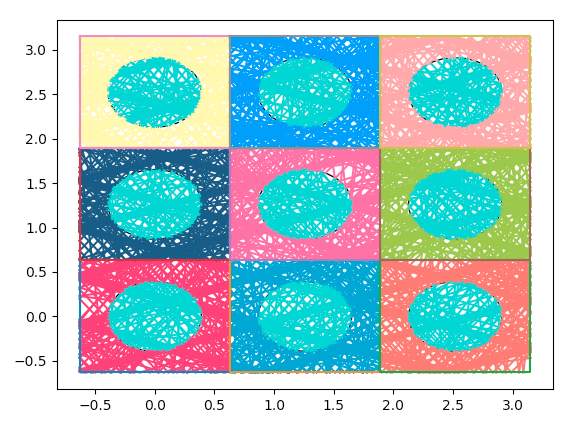
\includegraphics[width=0.8\textwidth]{raysPic}
  \caption{\label{fig:fig1}} Here is a picture of my pincell 3x3 with a lot of rays in it.
\end{figure}


\begin{figure}[H]
\centering
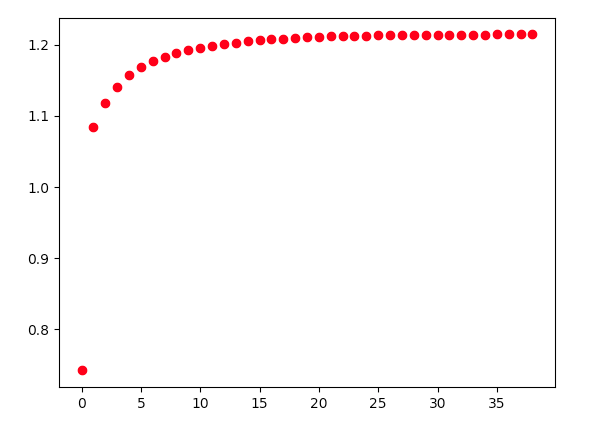
\includegraphics[width=0.8\textwidth]{keff_convergence}
  \caption{\label{fig:fig1}} This is my $k$ converging over the 38 iterations deemed necessary. The final $k$ value was 1.21465800448
\end{figure}


This ends up being significantly different from my OpenMC solution, which was apprxoimately 1.4 for my $k$ value. My CPM was terrible so I don't think I can compare it to that very well. \par~\par


For Dancoff, I tried to calculate 
\[C=1-\frac{\phi_0}{\phi}\]
for which I got 
\[C=1-\frac{17}{74}=0.77\]
My dancoff code is called the same way that my normal MOC code is called, which is by just running ``python dancoff\_moc.py''. In order to treat my pin as isolated, uncomment lines 355-356 and comment lines 359 and 360, and in order to treat as part of a lattice, do the opposite. Should run well. At the end of each iteration, it will print out flux $\phi$, and the cell that we are interested in is the is $\phi[4]$, for the center cell in this 3x3 lattice. Note that the material specifications that I made are defined in materials.py (like saying that the $\Sigma_t^F=10^5$.






\begin{figure}[H]
\centering
\includegraphics[width=0.4\textwidth]{sensitivity_1000Rays_200cmDist_VaryDeadzone.png}
\includegraphics[width=0.4\textwidth]{sensitivity_1000Rays_500cmDist_VaryDeadzone.png}
\includegraphics[width=0.4\textwidth]{sensitivity_1000Rays_VaryDist_50Deadzone.png}
\includegraphics[width=0.4\textwidth]{sensitivity_VaryRays_500cmDist_50Deadzone.png}
  \caption{\label{fig:fig1}} 
\end{figure}
For the sensititivity analysis part, I notice that varying deadzone length has an effect on shorter rays (2m rays), but has virtually no effect on $k$. Changing ray distance has a pretty significant effect on $k$, as does varying the number of rays run. Note that the difference between 100cm ray and 200cm ray is a lot more substantial than the difference between a 500cm ray and a 600cm ray.



%\begin{thebibliography}{9}
%\bibitem{nano3}
%  K. Grove-Rasmussen og Jesper Nygård,
%  \emph{Kvantefænomener i Nanosystemer}.
%  Niels Bohr Institute \& Nano-Science Center, Københavns Universitet
%
%\end{thebibliography}


\end{document}
